The client side is implemented as an Android application, \textit{DMDataGenerator}, that gathers location data for its users, interracts with the server and, if needed, it communicates a possible \textit{safe location} to the user.

Taking into consideration the fact that we have developed this client application as an easy way of testing the underlying management algorithm, there are multiple ways of using it, as a user but also as a developer:

\begin{itemize}
\item Generate data samples
\item Combine data samples into custom new ones
\item Replay samples
\item Choose preferences in terms of what means a \textit{safe location}
\item Choose friends
\end{itemize}

In the next paragraphs we will briefly describe each structural component of the client application and also the protocol used to communicate with the server.

\begin{wrapfigure}{R}{0.3\textwidth}
\centering
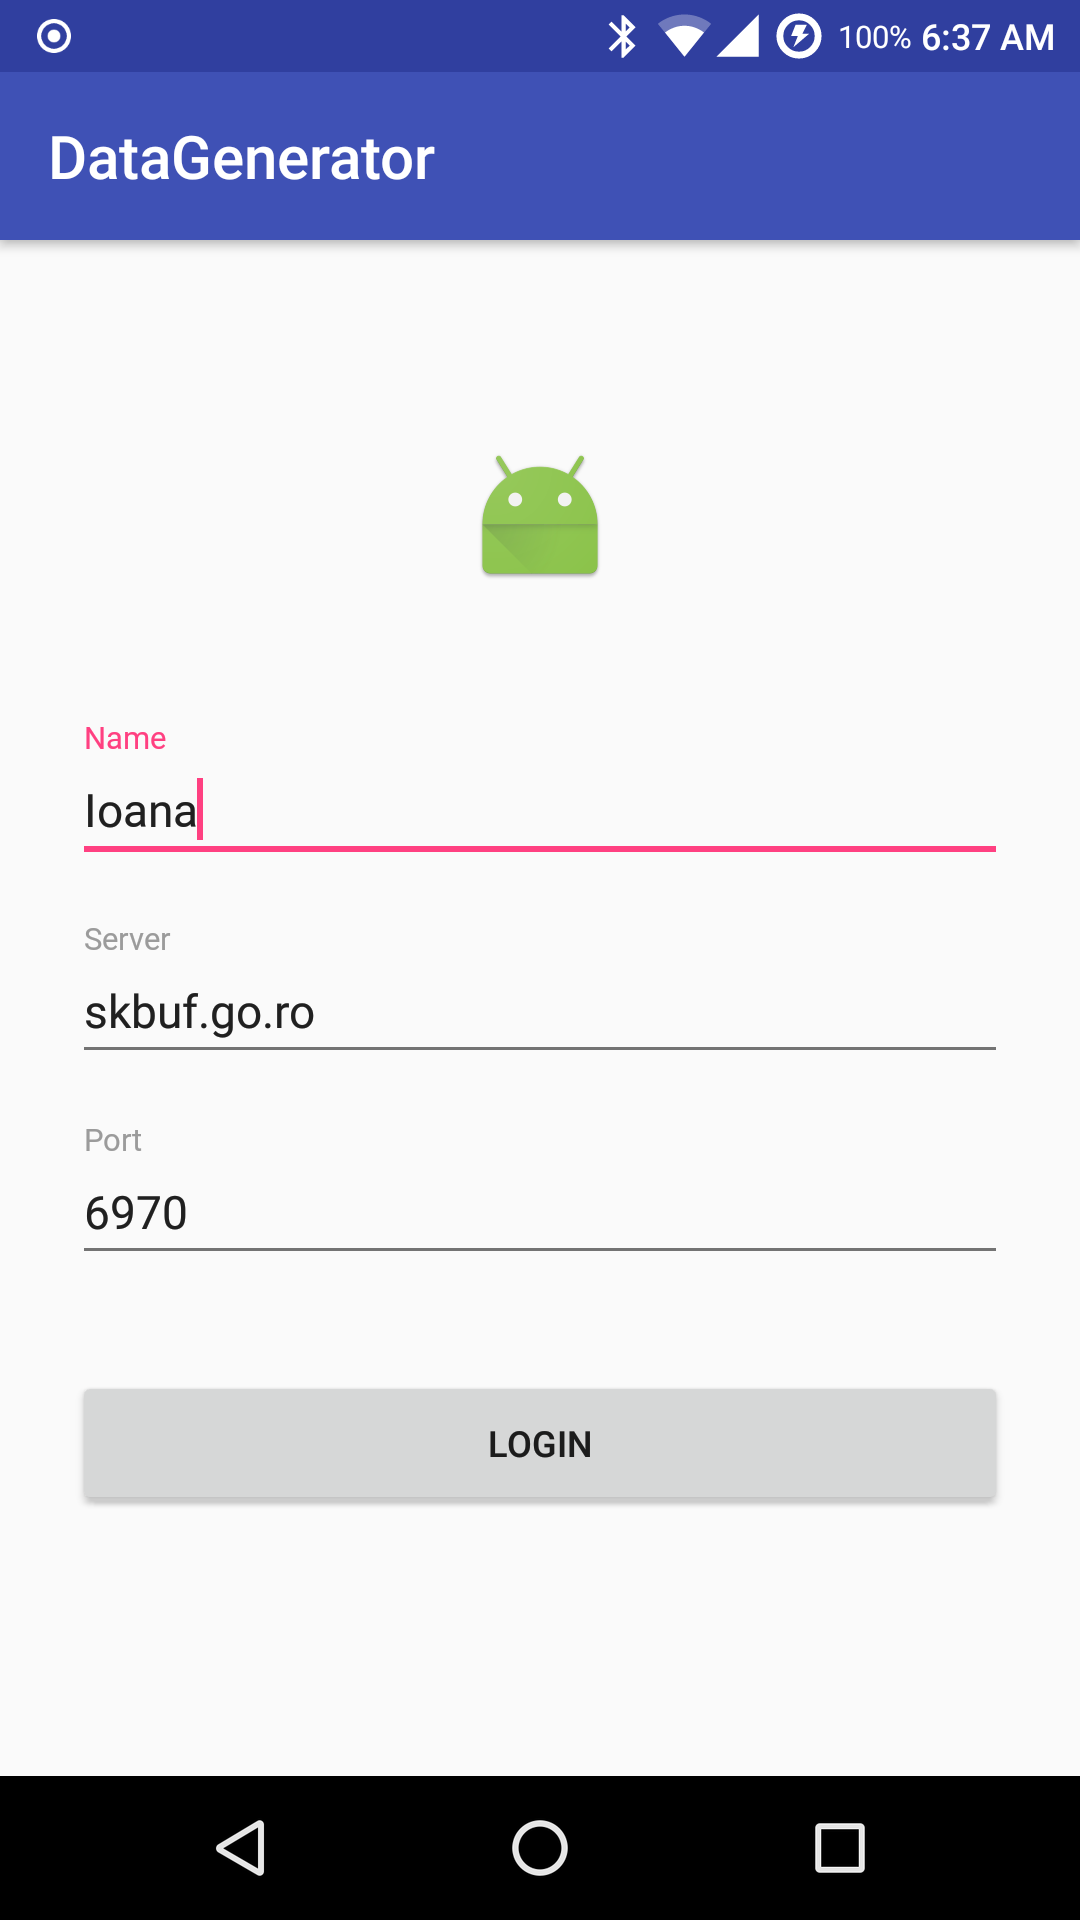
\includegraphics[scale=0.1]{login}
\caption{\label{fig:login}Login Activity}
\end{wrapfigure}

Using the \textit{Login Activity}, Figure \ref{fig:login}, an user can manually select the address of the server and also an username to be used throughout the application. 

\begin{wrapfigure}{R}{0.3\textwidth}
\centering
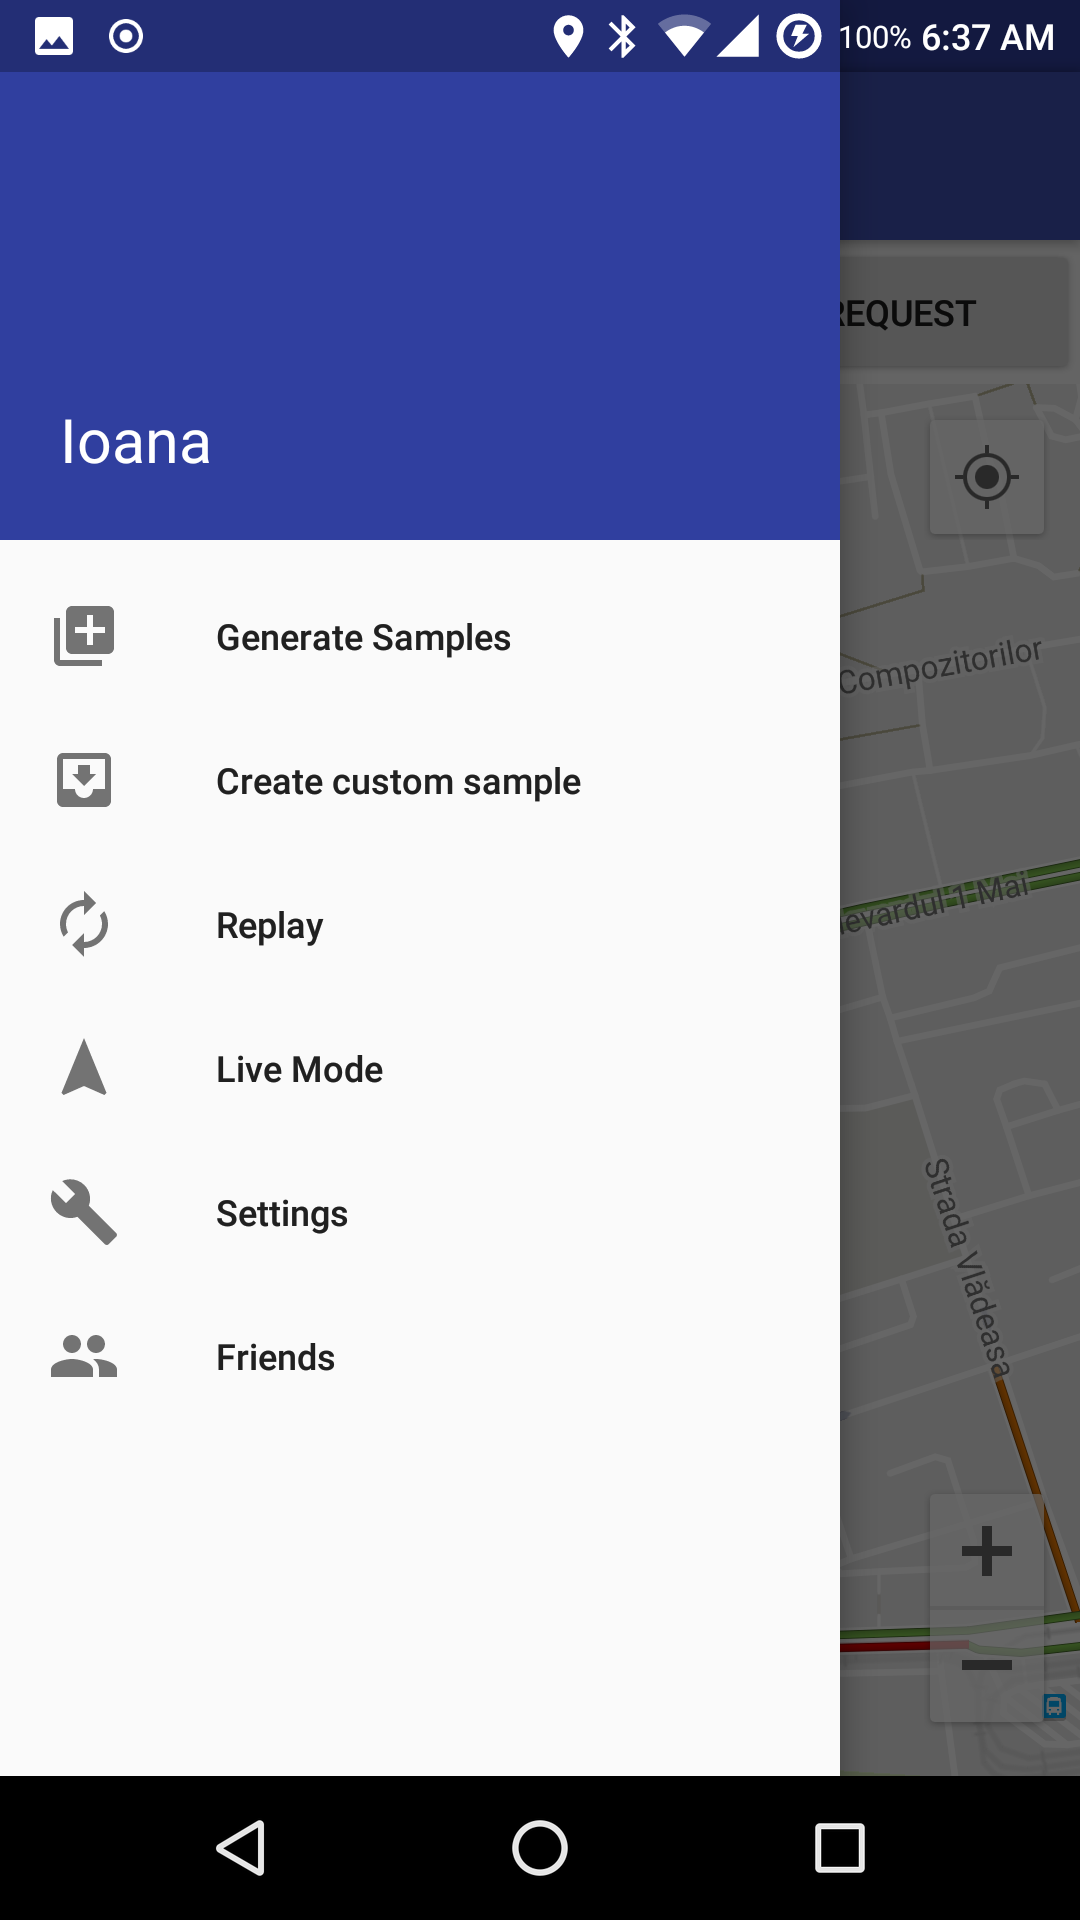
\includegraphics[scale=0.1]{menu}
\caption{\label{fig:menu} Menu sidebar}
\end{wrapfigure}

By pressing \textit{Login}, the user is redirected to the \textit{MainActivity}. There, using the options presented in the \textit{Menu Sidebar - Figure \ref{fig:menu}}, an user can easily navigate through features.

\begin{wrapfigure}{R}{0.3\textwidth}
\centering
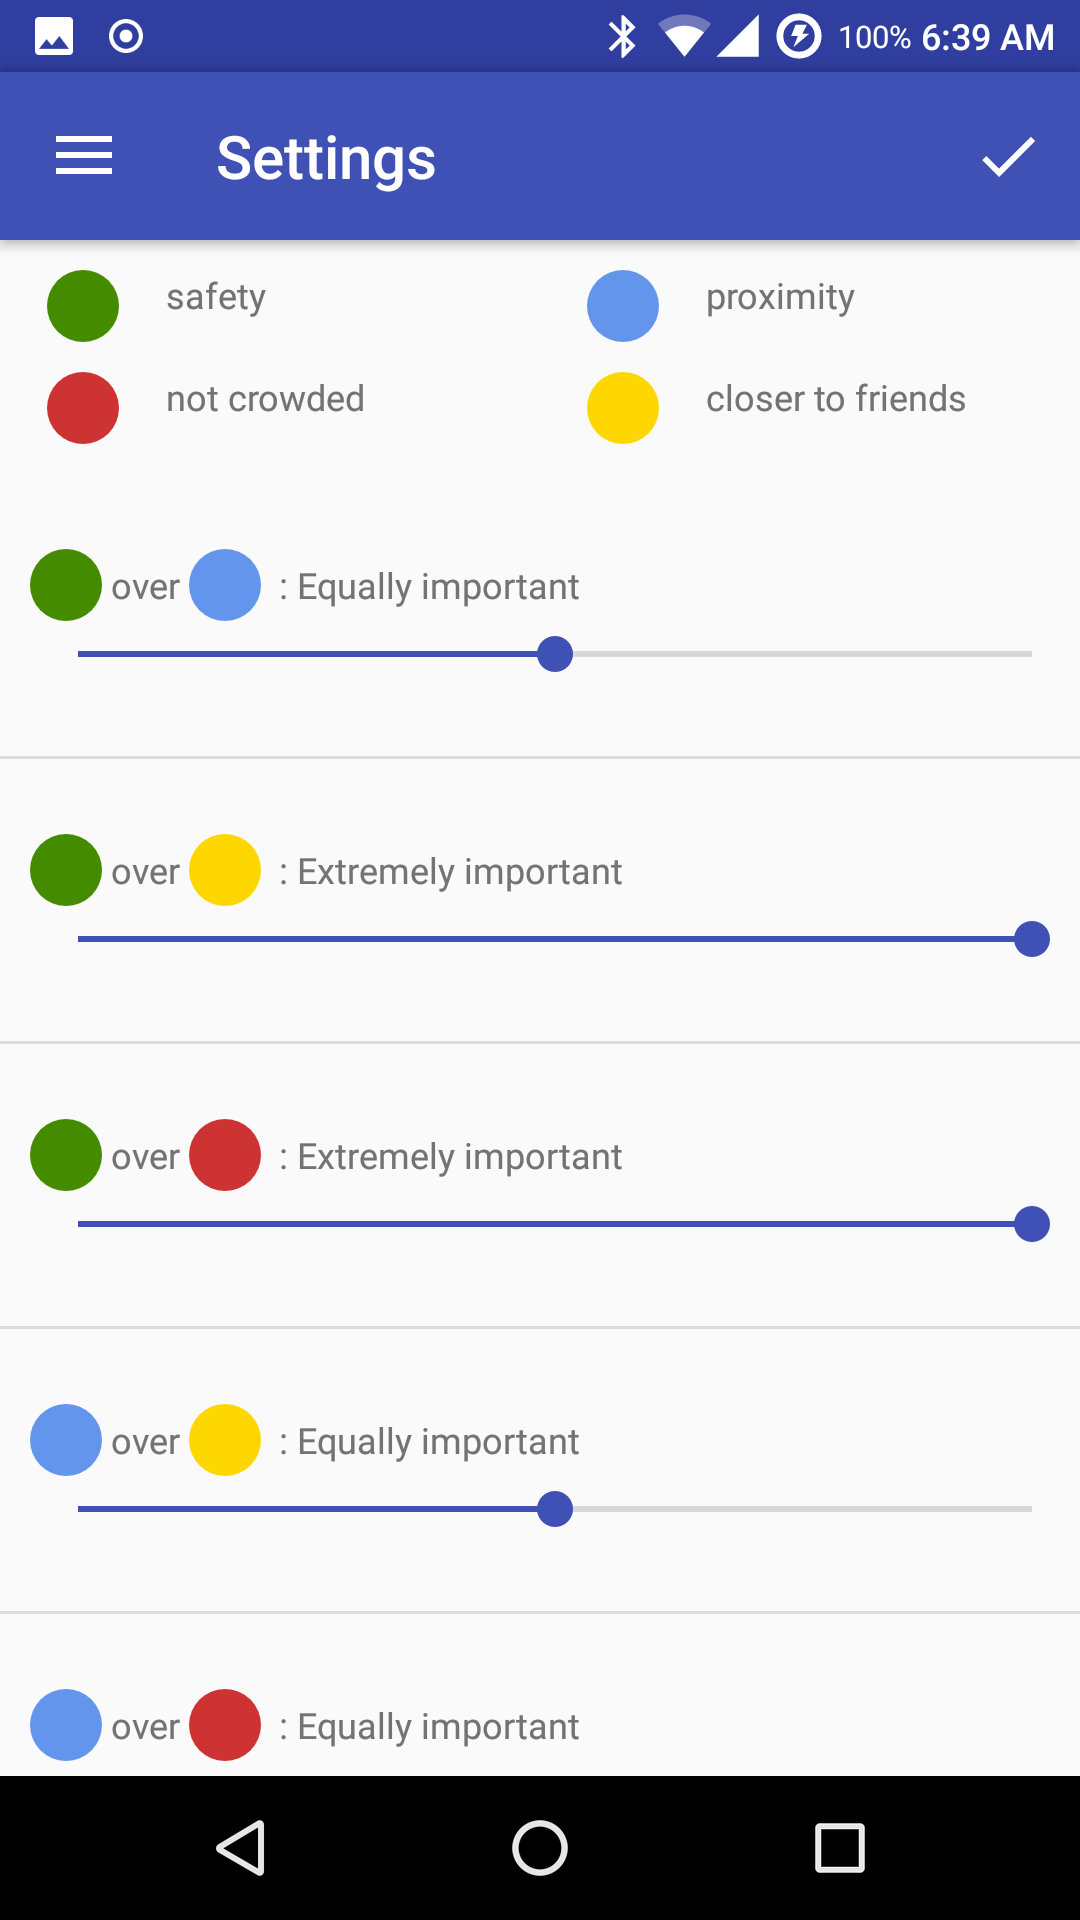
\includegraphics[scale=0.1]{settings}
\caption{\label{fig:settings}Settings Activity}
\end{wrapfigure}

Before trying to generate or manipulate data samples, an user must set its preferences using the menu item - \textit{Settings - Figure \ref{fig:settings}}.

As stated before in the Introduction - Chapter \ref{sec:introduction}, one can customize, depending on its preferences, the way a \textit{safe location} is defined.

Starting from the 4 criteria described above, one can specify the importance of one over another. And because consistency of preferences must be always met, an user can always verify if everything is in order using the check toolbar button.

\begin{wrapfigure}{R}{0.3\textwidth}
\centering
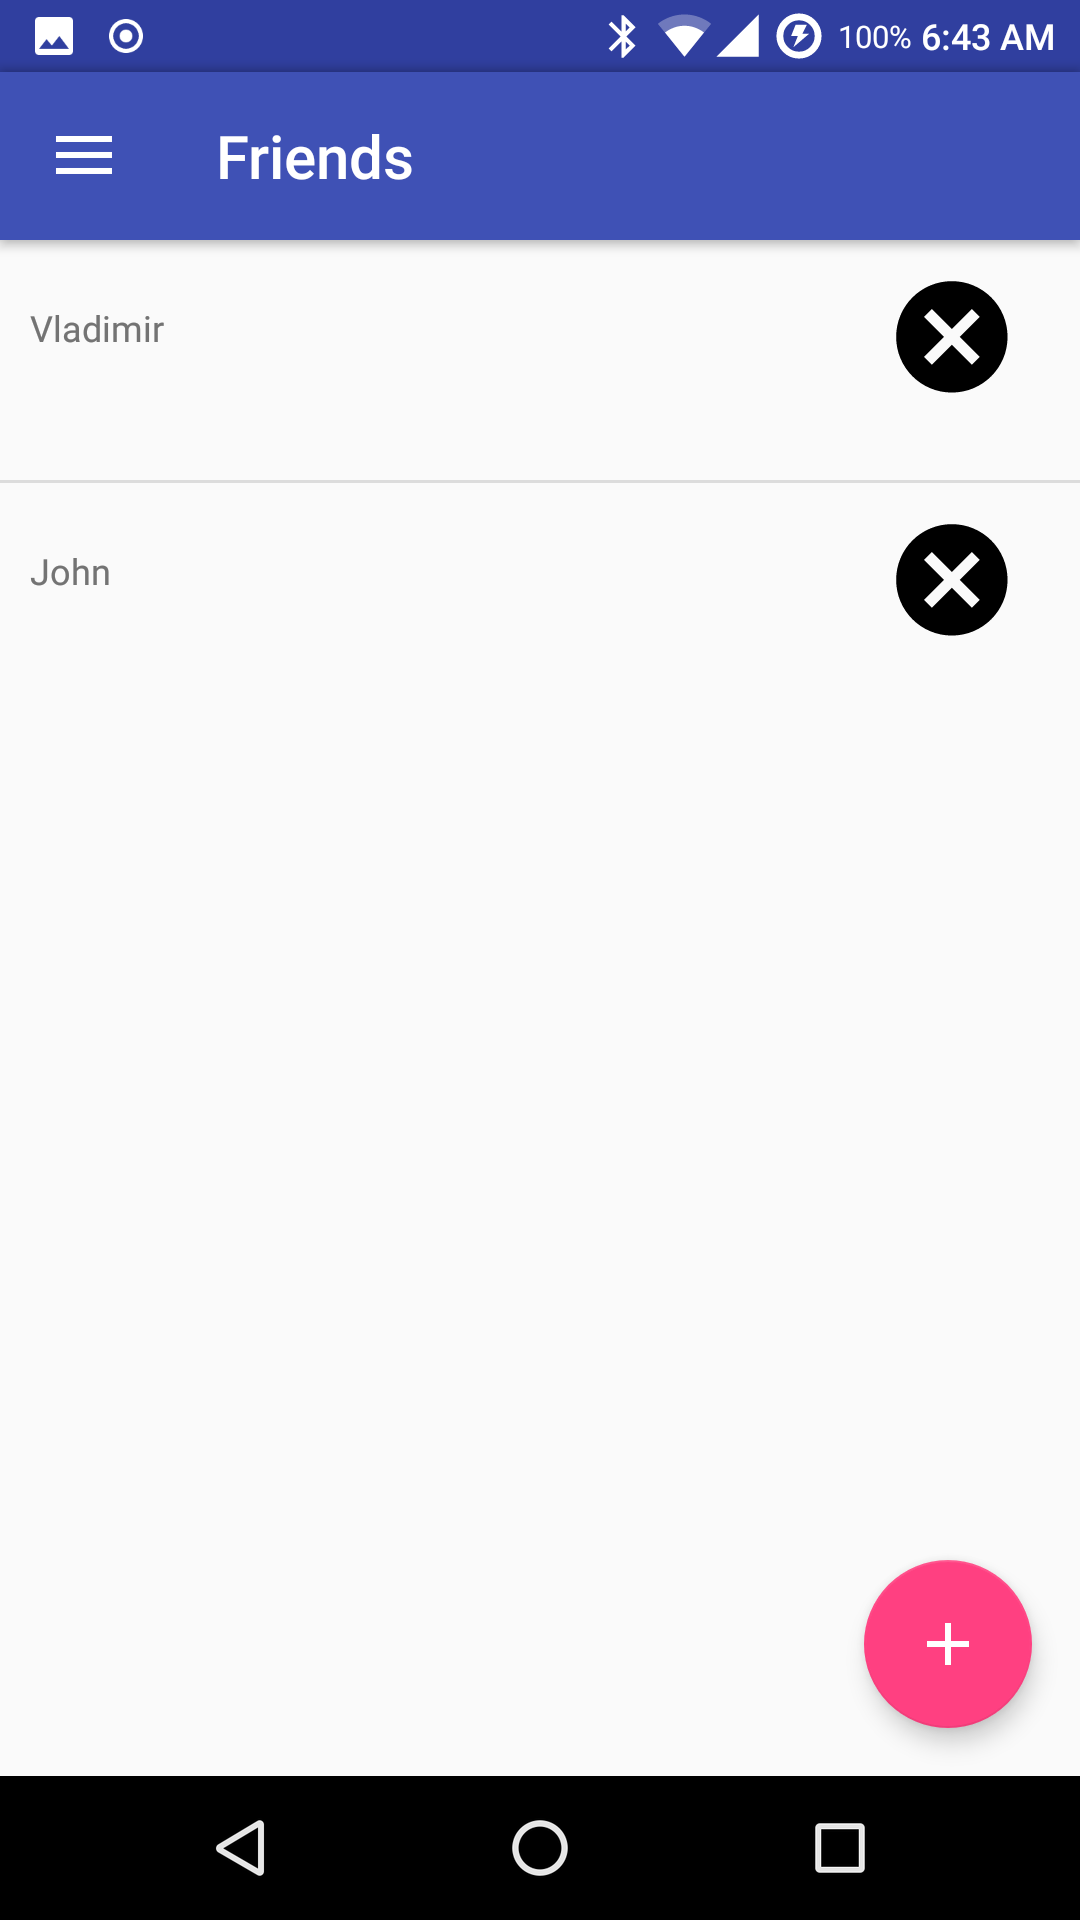
\includegraphics[scale=0.1]{friends}
\caption{\label{fig:friends}Friends Activity}
\end{wrapfigure}

\textit{Proximity to friends} is one of the criteria used to evaluate a possible \textit{safe spot} thus specifiying other users trated as friends is possible using the \textit{Friends Activity - Figure \ref{fig:friends}}.

When interracting with the server, user preferences and also friends names are transformed into JSON formatted messages, as explained above. In this specific case, message types \textit{safe-location-preferences} and \textit{friends} are used.

\begin{wrapfigure}{R}{0.3\textwidth}
\centering
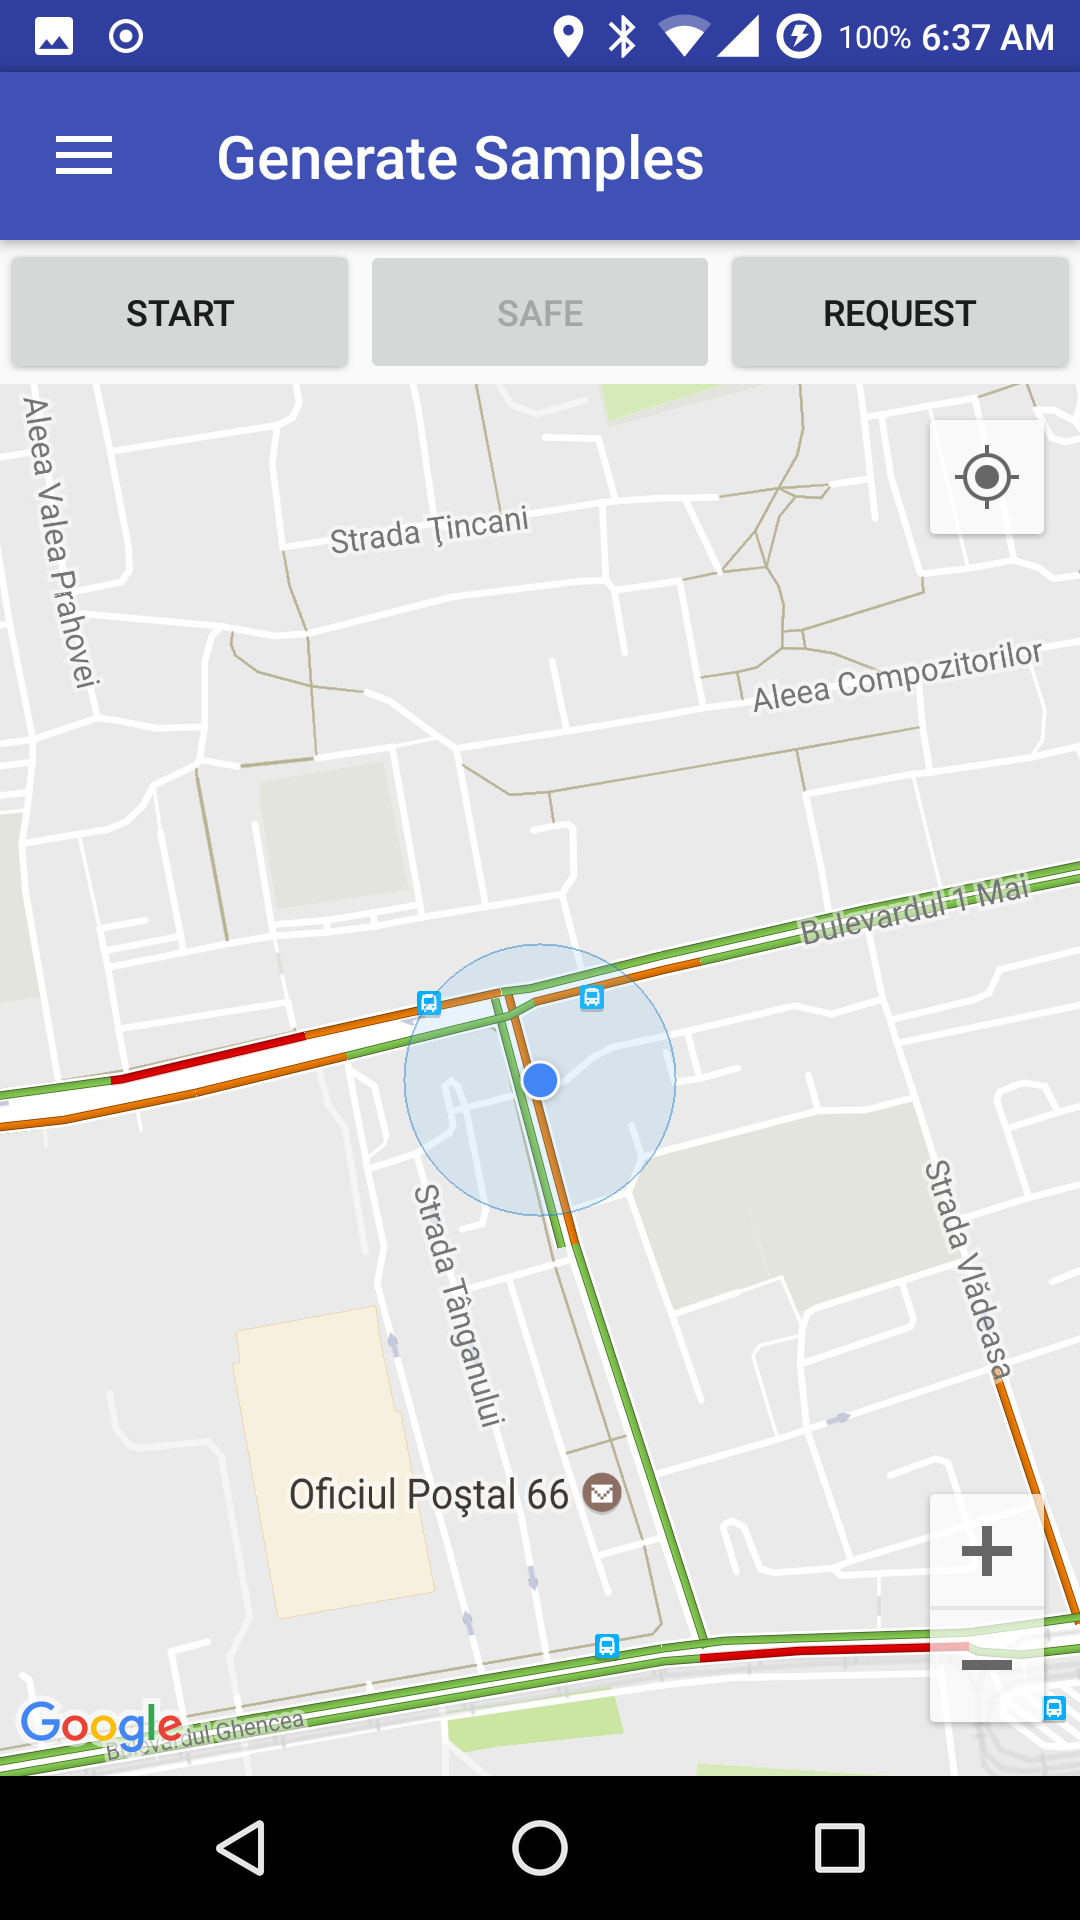
\includegraphics[scale=0.1]{generate}
\caption{\label{fig:generate}Generate Sample Activity}
\end{wrapfigure}

Using \textit{Generate Sample Activity - Figure \ref{fig:generate}}, one can create data samples based on location updates provided by GoogleAPIs. The user is given the option of announcing that he/she found a \textit{safe spot} or to request one from its peers. Upon termination, a text file with the \textit{sample-timestamp-username} format is created on the external storage (/sdcard/DMDataGenerator-Samples).

\lstset{
    string=[s]{"}{"},
    stringstyle=\color{blue},
    comment=[l]{:},
    commentstyle=\color{black},
}

%\begin{lstlisting}
%{"msgtype":"delete-clients"}
%{"msgtype":"delete-safe-locations"}
%{"msgtype":"friends","name":"111","friends":["22"]}
%{"msgtype":"safe-location-preferences","name":"111","criteria":["safety","proximity","closeToFriends","notCrowded"],"pairwiseComparisons":[4.0,4.0,4.0,1.0,1.0,1.0]}
%{"msgtype":"client-location","name":"111","timestamp":998,"latitude":44.418954,"longitude":26.0436168}
%{"msgtype":"client-location","name":"111","timestamp":1998,"latitude":44.4189502,"longitude":26.0436203}
%{"msgtype":"safe-location-request","timestamp":43752,"name":"111"}
%{"msgtype":"safe-location","name":"111","timestamp":7389,"latitude":44.4188103,"longitude":26.0443281}
%\end{lstlisting}


\begin{wrapfigure}{R}{0.3\textwidth}
\centering
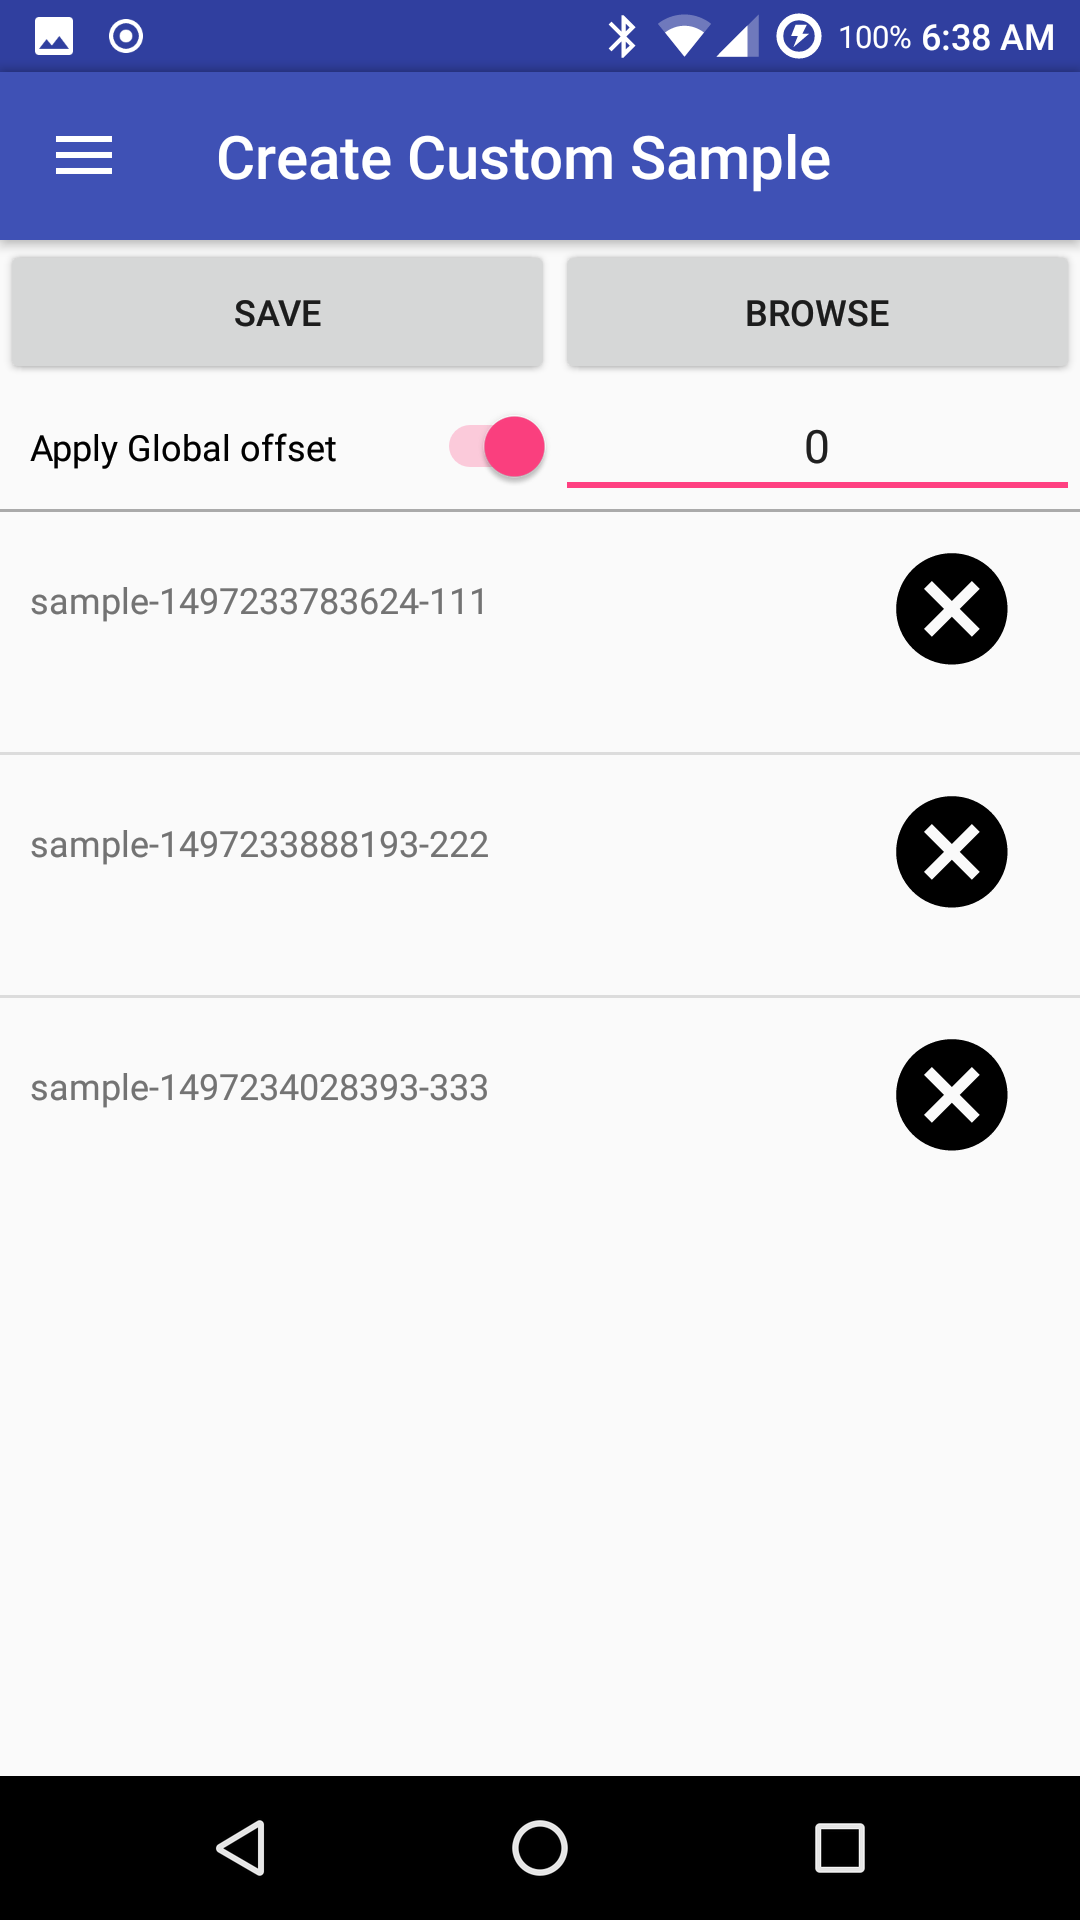
\includegraphics[scale=0.1]{custom}
\caption{\label{fig:custom}Create Custom Sample Activity}
\end{wrapfigure}

\begin{wrapfigure}{R}{0.3\textwidth}
\centering
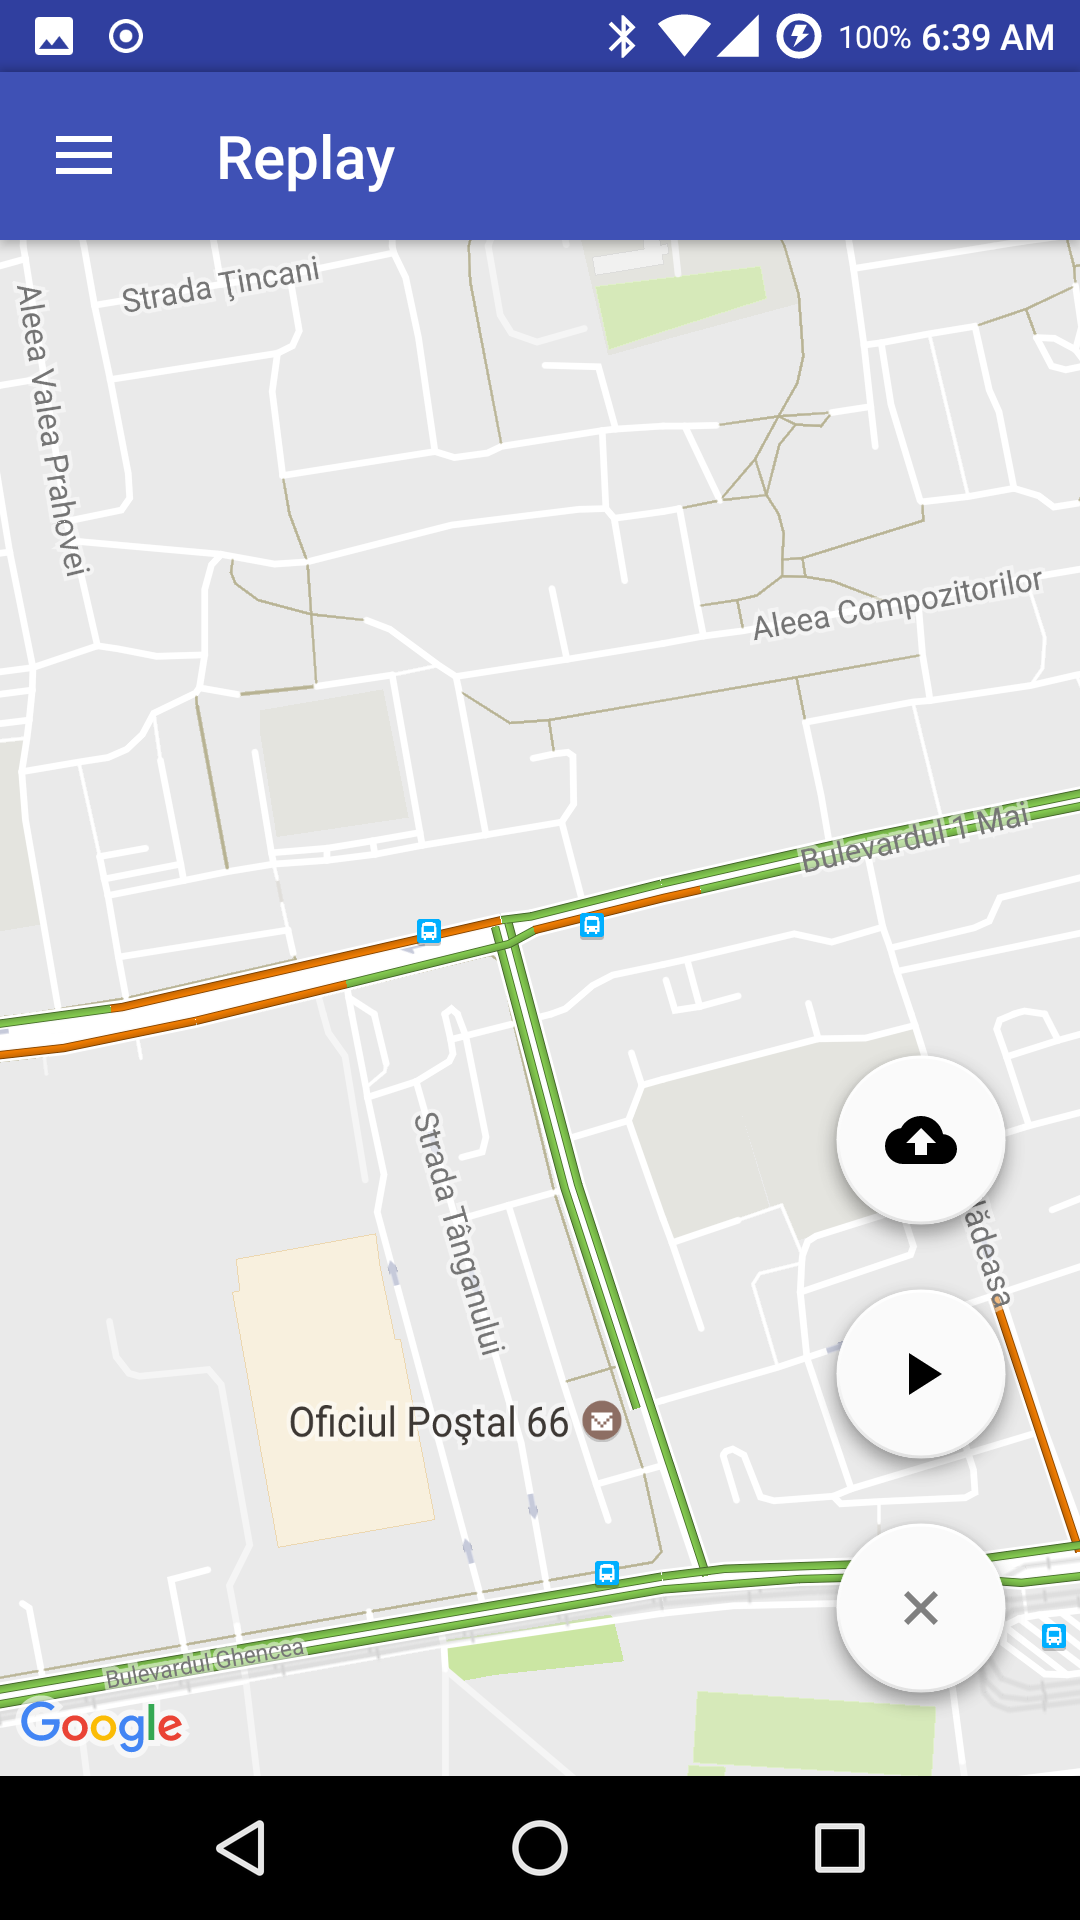
\includegraphics[scale=0.1]{replay}
\caption{\label{fig:replay}Replay Activity}
\end{wrapfigure}

\begin{wrapfigure}{R}{0.3\textwidth}
\centering
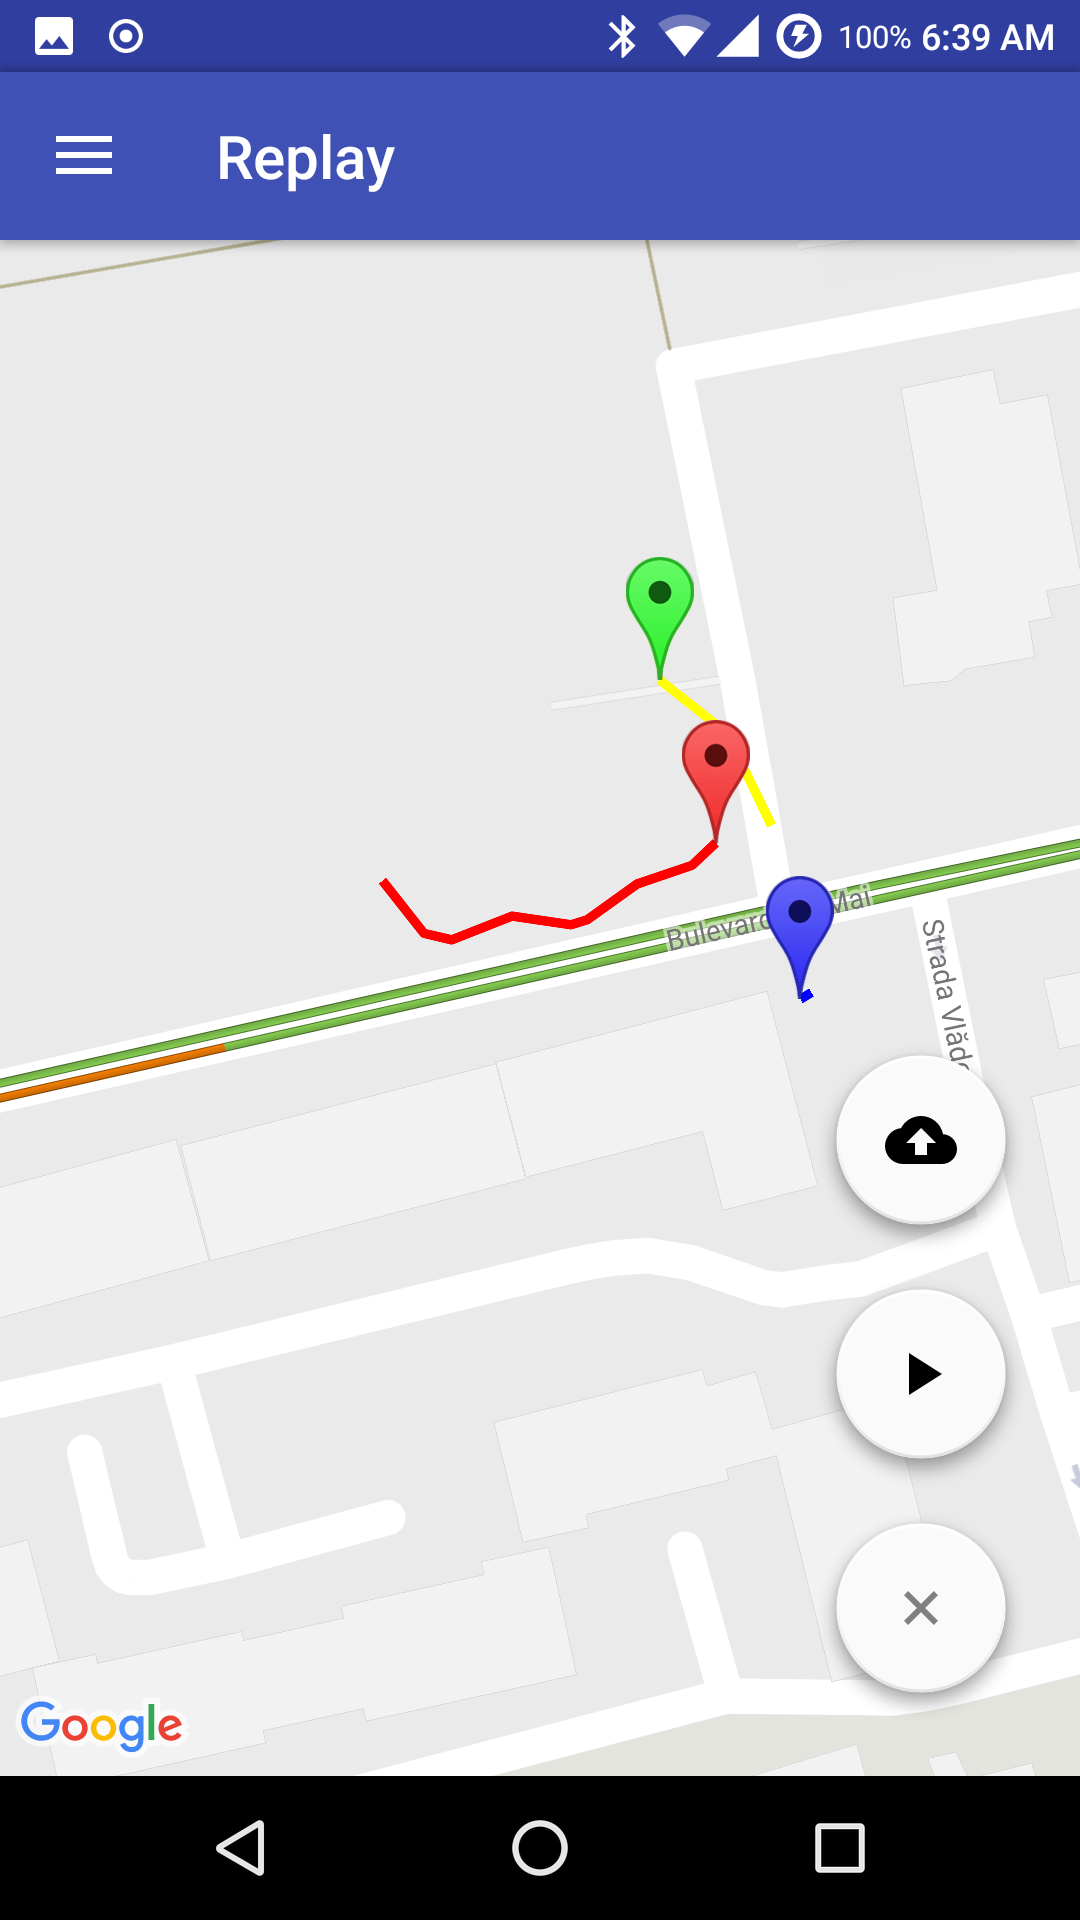
\includegraphics[scale=0.1]{replayfound}
\caption{\label{fig:replayfround}Replay Activity with Safe place found}
\end{wrapfigure}
